\documentclass[conference]{IEEEtran}
\IEEEoverridecommandlockouts
% The preceding line is only needed to identify funding in the first footnote. If that is unneeded, please comment it out.
\usepackage{cite}
\usepackage{amsmath,amssymb,amsfonts}
\usepackage{algorithmic}
\usepackage{graphicx}
\usepackage{textcomp}
\usepackage{xcolor}
\usepackage{minted}

\def\BibTeX{{\rm B\kern-.05em{\sc i\kern-.025em b}\kern-.08em
    T\kern-.1667em\lower.7ex\hbox{E}\kern-.125emX}}
\begin{document}

\title{SE 380 P3}

\author{\IEEEauthorblockN{1\textsuperscript{st} Bilal Khan}
\IEEEauthorblockA{b54khan@uwaterloo.ca}
\and
\IEEEauthorblockN{2\textsuperscript{nd} Bohdan Hrotovytskyy}
\IEEEauthorblockA{bhrotovy@uwaterloo.ca}
}

\maketitle

\section{Item 1}

We can find the controllable canonical state space form of this transfer function by reading off from the transfer function:

\begin{align*}
    \dot{x_1} &= \begin{bmatrix}
        0 & 1 \\
        -0.005 & -1.05 \\
    \end{bmatrix}
    x_1 +
    \begin{bmatrix}
        0 \\
        1 \\
    \end{bmatrix}
    u_1 \\
    y_1 &= \begin{bmatrix}
        0.53 & 0 \\
    \end{bmatrix}
    x_1 +
    \begin{bmatrix}
        0 \\
    \end{bmatrix}
    u_1 \\
    \dot{x_2} &= \begin{bmatrix}
        0 & 1 \\
        -0.005 & -1.05 \\
    \end{bmatrix}
    x_2 +
    \begin{bmatrix}
        0 \\
        1 \\
    \end{bmatrix}
    u_2 \\
    y_2 &= \begin{bmatrix}
        0.53 & 0 \\
    \end{bmatrix}
    x_2 +
    \begin{bmatrix}
        0 \\
    \end{bmatrix}
    u_2 \\
\end{align*}

\section{Item 2}

Solving the overshoot equation for $\zeta$ using wolfram alpha gives us $\zeta \approx 0.78$. This gives us $\omega_n = 1.28$ that satisfies the settling time. The desired closed loop poles are $-0.78 \pm 1.28i$. The desired characteristic polynomial is:

\begin{align*}
    P(\lambda) &= (\lambda - (-0.78 + 1.28i)) (\lambda - (-0.78 - 1.28i))  \\
    &= (\lambda + 0.78 - 1.28i) (\lambda + 0.78 + 1.28i) \\
    &= \lambda^2 + 1.56 \lambda + 2.24 \\
\end{align*}

Using Thm 3 from the notes, the $K_1$ and $K_2$ values are then given by:

\begin{align*}
    1.05 + a &= 1.56 \\
    0.005 + b &= 2.24 \\
\end{align*}

$K_1 = K_2 = [2.235, 0.51]^T$

\section{Item 3}

\begin{minted}[breaklines]{python}
import numpy as np
class Controller:    
    def __init__(self, delta_t):
        self.y = np.zeros((2, 1))
        self.delta_t = delta_t
        self.K_1 = self.K_2 = np.array([2.235, 0.51])
    def calculate_acceleration(self, y):
        y_dot = (y - self.y) / self.delta_t
        self.y = y
        x_1 = np.array([y[0], y_dot[0]])
        x_2 = np.array([y[1], y_dot[1]])
        u_1 = -np.dot(self.K_1, x_1)
        u_2 = -np.dot(self.K_2, x_2)
        return np.array([u_1, u_2]).reshape(2, 1)
\end{minted}

\section{Item 4}

Computing the controllable canonical state space form of the filter gives us:

\begin{align*}
    A_f &= \begin{bmatrix}
        0 & 1 & 0 \\
        0 & 0 & 1 \\
        -1000 & -300 & -30 \\
    \end{bmatrix} \\
    B_f &= \begin{bmatrix}
        0 \\
        0 \\
        1 \\
    \end{bmatrix} \\
    C_f &= \begin{bmatrix}
        1000 & 0 & 0 \\
    \end{bmatrix} \\
    D_f &= 0 \\
\end{align*}

We then implement this in code in controller.py (lines 20-40) following the hint

\section{Item 5}

The code for this can be found in main.py. The plots are shown below:

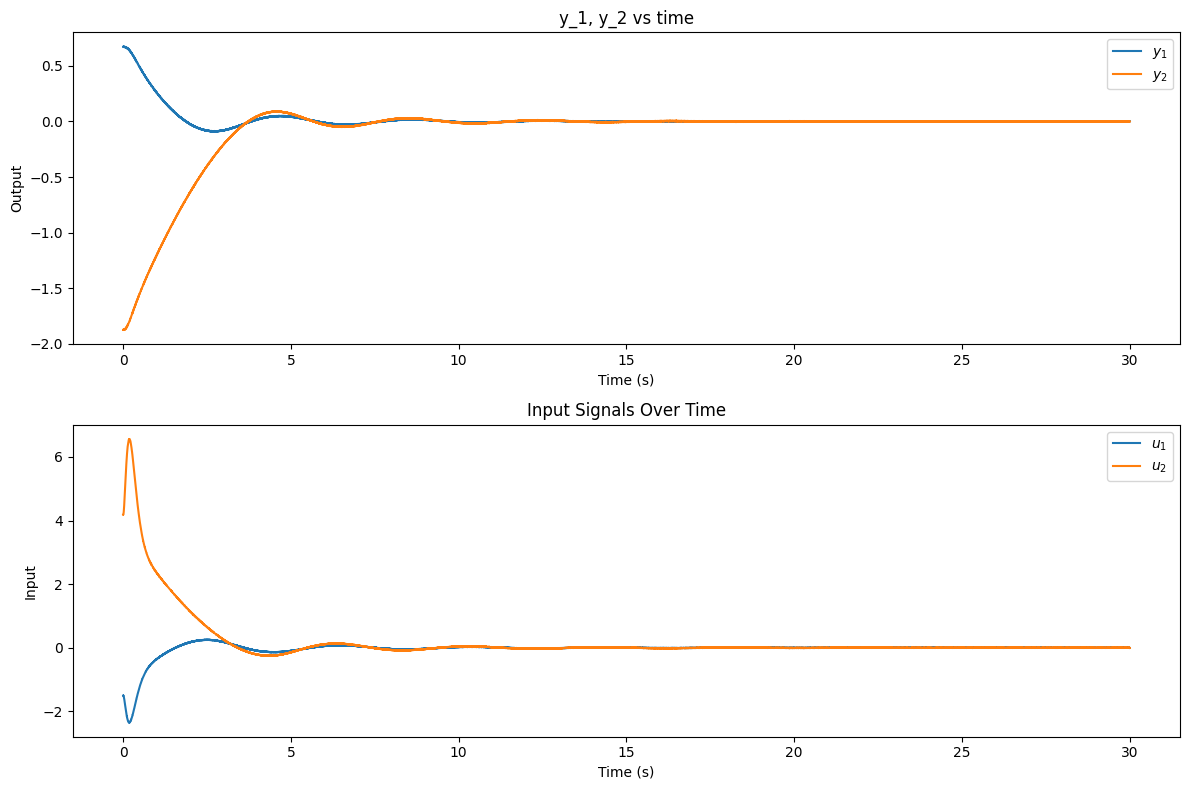
\includegraphics[width=500pt]{p3.png}

\end{document}
